\section{Thiết kế hệ thống}
\label{sec:design}

\subsection{Mục tiêu thiết kế}
\label{subsec:design-goals}

Mục tiêu của chương này là chuyển hoá kết quả phân tích ở Chương~\ref{sec:analysis} thành các quyết định thiết kế cụ thể ở mức:
(i) kiến trúc tổng thể client--server và triển khai;
(ii) thiết kế mô-đun backend và ranh giới trách nhiệm;
(iii) thiết kế dữ liệu (progression/\allowbreak state và game configuration);
(iv) thiết kế giao tiếp (HTTP/\allowbreak WebSocket) và quy ước dữ liệu;
(v) thiết kế các cơ chế đảm bảo nhất quán, bảo mật và quan sát hệ thống;
(vi) thiết kế giao diện UI/\allowbreak UX ở mức tham chiếu để đối chiếu với luồng nghiệp vụ và API.

Trong giai đoạn 1, thiết kế ưu tiên:
\begin{itemize}
    \item \textbf{Tính đúng đắn và nhất quán}: các thay đổi ảnh hưởng tiến trình (reward/\allowbreak currency/\allowbreak gacha/\allowbreak checkpoint, nâng cấp, tiêu hao vật phẩm) phải được server xác nhận.
    \item \textbf{Tính mô-đun}: phân tách rõ theo phân hệ (auth, profile, character, inventory, equipment, skills, combat, gacha, island, admin).
    \item \textbf{Tính data-driven cho cấu hình}: tách dữ liệu cấu hình gameplay khỏi mã nguồn; hỗ trợ quản trị và thay đổi nhanh.
    \item \textbf{Phù hợp phạm vi đồ án}: triển khai ở mức hợp lý (single deployment có thể chạy được), nhưng vẫn giữ được hướng mở rộng.
\end{itemize}

% ==============================================================
\subsection{Kiến trúc tổng thể và triển khai}
\label{subsec:design-architecture}

\subsubsection{Tổng quan triển khai}
\label{subsubsec:design-deploy-overview}

Hệ thống được tổ chức thành 3 lớp chính: \textit{Client Devices}, \textit{Backend Infrastructure} và \textit{Data \& Storage}. Hình~\ref{fig:deploy-diagram} mô tả các thành phần và đường giao tiếp chính.

\begin{figure}[H]
    \centering
    \includegraphics[width=0.95\textwidth]{Images/DeployDiagram.png}
    \caption{Sơ đồ triển khai tổng quan hệ thống}
    \label{fig:deploy-diagram}
\end{figure}

Các thành phần cốt lõi:
\begin{itemize}
    \item \textbf{Game Client (Unity)}: hiển thị đồ hoạ, UI, thu thập input; giao tiếp với server qua HTTPS và WebSocket.
    \item \textbf{API Server (NestJS)}: lớp ứng dụng xử lý REST API, đồng thời cung cấp kênh real-time (WebSocket gateway) cho phiên chơi.
    \item \textbf{Job Worker}: xử lý tác vụ nền theo lịch (ví dụ: mail hệ thống, sự kiện, tổng hợp log, dọn dẹp dữ liệu runtime).
    \item \textbf{MongoDB (Primary DB)}: lưu dữ liệu tiến trình bền vững và các collections cấu hình.
    \item \textbf{Redis (Cache \& Pub/\allowbreak Sub)}: lưu cache/\allowbreak session runtime hoặc pub-sub khi mở rộng nhiều instance.
    \item \textbf{MinIO (Object Storage)}: lưu trữ tệp và asset bundle (nếu áp dụng); client tải qua presigned URL.
\end{itemize}

\subsubsection{Nguyên tắc server-authoritative}
\label{subsubsec:design-server-authoritative}

Thiết kế áp dụng nguyên tắc \textbf{server-authoritative} cho các tác vụ ảnh hưởng tiến trình và công bằng:
\begin{itemize}
    \item Client chỉ gửi \textbf{ý định} (intent), không gửi trạng thái ``đã xảy ra'' như ``đã trúng đòn'' hay ``đã nhận item''.
    \item Server kiểm tra luật (cooldown, tài nguyên, điều kiện tham gia, dung lượng inventory, điều kiện skill) và chỉ khi hợp lệ mới ghi dữ liệu.
    \item Các giao dịch reward/\allowbreak currency/\allowbreak gacha/\allowbreak checkpoint, nâng cấp trang bị/\allowbreak kỹ năng được coi là \textbf{giao dịch nghiệp vụ} và phải có log/\allowbreak audit để truy vết.
\end{itemize}
Các quyết định này giúp giảm rủi ro gian lận và tăng tính nhất quán trong môi trường online \cite{gaffer-networking,moriarty-networked}.

\subsubsection{Phân tách giao tiếp: HTTP và WebSocket}
\label{subsubsec:design-protocols}

\paragraph{HTTP/\allowbreak REST} được dùng cho:
\begin{itemize}
    \item đăng ký/\allowbreak đăng nhập, khôi phục tài khoản;
    \item quản lý profile/\allowbreak nhân vật;
    \item tải dữ liệu meta (inventory, equipment, skills, island state, NPC collection);
    \item thao tác quản trị (admin) và các tác vụ không yêu cầu độ trễ thấp.
\end{itemize}

\paragraph{WebSocket} được dùng cho:
\begin{itemize}
    \item tham gia instance/\allowbreak room và vòng lặp chiến đấu real-time;
    \item gửi input (move/\allowbreak attack/\allowbreak cast/\allowbreak dodge) theo nhịp;
    \item nhận snapshot/\allowbreak event từ server để hiển thị mượt.
\end{itemize}

% ==============================================================
\subsection{Thiết kế mô-đun backend}
\label{subsec:design-backend-modules}

Backend được tổ chức theo phong cách module hoá của NestJS \cite{nest-docs}. Mỗi mô-đun tương ứng một phân hệ nghiệp vụ và sở hữu ranh giới dữ liệu rõ ràng. Bảng~\ref{tab:module-map} tóm tắt các mô-đun chính.

\begin{table}[H]
\centering
\renewcommand{\arraystretch}{1.2}
\setlength{\tabcolsep}{6pt}
\begin{tabularx}{\textwidth}{|L{3.25cm}|Y|L{4.1cm}|}
\hline
\textbf{Mô-đun} & \textbf{Trách nhiệm chính} & \textbf{Dữ liệu/\allowbreak Collection liên quan} \\
\hline
Auth Module & Đăng ký/\allowbreak đăng nhập; cấp và xác thực token; chính sách role & USER, SESSION\_\allowbreak RUNTIME \\
\hline
Profile Module & Tạo/\allowbreak chọn profile; cập nhật last\_played; thiết lập profile & GAME\_\allowbreak PROFILE \\
\hline
Character Module & Tạo/\allowbreak chọn/\allowbreak xoá nhân vật; quản lý level/\allowbreak EXP; base stats, appearance & CHARACTER \\
\hline
Inventory Module & Quản lý slot, stack, currency; dùng vật phẩm; cập nhật reward & INVENTORY, CONFIG\_\allowbreak ITEM \\
\hline
Equipment Module & Trang bị theo slot; đồng bộ durability/\allowbreak enhance; tính chỉ số cộng thêm & CHARACTER\_\allowbreak EQUIPMENT, CONFIG\_\allowbreak ITEM \\
\hline
Skill Module & Điểm kỹ năng; learned skills; hotbar; nâng cấp skill & CHARACTER\_\allowbreak SKILLS, CONFIG\_\allowbreak SKILL \\
\hline
Combat Module & Tham gia tower/\allowbreak dungeon/\allowbreak arena; quản lý instance/\allowbreak room; tick loop; snapshot & SESSION\_\allowbreak RUNTIME, (runtime state) \\
\hline
Gacha Module & Banner, rate, pity, exchange; xử lý duplicate; ghi lịch sử & NPC\_\allowbreak COLLECTION, (gacha history), config rates \\
\hline
Island Module & Tài nguyên đảo; xây/\allowbreak nâng cấp công trình; timer; layout; gán worker & PERSONAL\_\allowbreak ISLAND, CONFIG\_\allowbreak BUILDING \\
\hline
NPC Module & Bộ sưu tập NPC; levelling/\allowbreak star/\allowbreak friendship; job/\allowbreak assignment & NPC\_\allowbreak COLLECTION \\
\hline
Admin Module & Ban/\allowbreak unban; system mail; log viewer; event config; quản trị cấu hình & USER, (mail/\allowbreak event/\allowbreak log), CONFIG\_\allowbreak * \\
\hline
Config Module & Nạp và cung cấp truy xuất cấu hình; versioning; cache & CONFIG\_\allowbreak * (static) \\
\hline
\end{tabularx}
\caption{Bản đồ mô-đun backend và dữ liệu liên quan}
\label{tab:module-map}
\end{table}

\subsubsection{Các thành phần dùng chung (cross-cutting)}
\label{subsubsec:design-crosscutting}

Để giảm trùng lặp và tăng tính nhất quán, hệ thống dùng các thành phần dùng chung:
\begin{itemize}
    \item \textbf{Validation}: kiểm tra input cho REST và WebSocket (schema/\allowbreak DTO) để chặn dữ liệu sai từ đầu.
    \item \textbf{Error handling}: chuẩn hoá mã lỗi và thông điệp lỗi; đảm bảo client có thể hiển thị đúng trạng thái UI (loading/\allowbreak error/\allowbreak disabled).
    \item \textbf{Logging \& audit}: log request, log nghiệp vụ (reward/\allowbreak gacha/\allowbreak equip/\allowbreak skill-up/\allowbreak admin action), kèm correlation id.
    \item \textbf{Rate limit / anti-spam}: giới hạn tần suất với endpoint nhạy cảm (login, gacha) và message real-time (input spam).
\end{itemize}

% ==============================================================
\subsection{Thiết kế dữ liệu}
\label{subsec:design-data}

\subsubsection{Nguyên tắc thiết kế dữ liệu}
\label{subsubsec:design-data-principles}

Hệ thống dữ liệu được chia thành 2 nhóm:
\begin{itemize}
    \item \textbf{Progression/\allowbreak State (động)}: dữ liệu người chơi thay đổi theo thời gian (profile, character, inventory, equipment, skills, island, NPC, pity, lịch sử gacha).
    \item \textbf{Game Configuration (tĩnh)}: dữ liệu định nghĩa và thông số gameplay (item/\allowbreak building/\allowbreak skill/\allowbreak rates/\allowbreak formulas).
\end{itemize}

Với MongoDB, thiết kế ưu tiên:
\begin{itemize}
    \item \textbf{Embed} khi dữ liệu có vòng đời gắn chặt với thực thể cha và thường được tải cùng nhau (ví dụ: base\_stats/\allowbreak resources/\allowbreak appearance nhúng trong CHARACTER; items nhúng trong INVENTORY; buildings nhúng trong PERSONAL\_ISLAND; skill list/\allowbreak hotbar nhúng trong CHARACTER\_SKILLS; từng slot trang bị nhúng trong CHARACTER\_EQUIPMENT).
    \item \textbf{Reference} khi dữ liệu là định nghĩa tĩnh dùng chung (CONFIG\_ITEM/\allowbreak CONFIG\_BUILDING/\allowbreak CONFIG\_SKILL) hoặc cần tái sử dụng giữa nhiều thực thể.
\end{itemize}

\subsubsection{Mô hình thực thể chính (ERD mức logic)}
\label{subsubsec:design-erd}

Trong phạm vi báo cáo, ERD được trình bày ở mức logic để làm rõ quan hệ 1:1, 1:N và các liên kết tham chiếu tới cấu hình. Các ``STRUCT\_*'' trong ERD đại diện cho \textbf{embedded document} (struct nhúng), không phải collection độc lập.

\begin{lstlisting}
erDiagram
    %% ==========================================
    %% 1. IDENTITY MODULE
    %% ==========================================
    USER {
        ObjectId _id PK
        string username
        string email
        string password_hash
        string role
        enum status
        date created_at
        date last_login
        object settings "Embed: OBJECT_USER_SETTINGS"
    }

    OBJECT_USER_SETTINGS {
        float master_volume
        float sfx_volume
        string language_code
        boolean notifications_enabled
    }

    GAME_PROFILE {
        ObjectId _id PK
        ObjectId user_id FK
        string profile_name
        string server_id
        date created_at
        date last_played
        object preferences "Embed: Local Game Settings"
    }

    SESSION_RUNTIME {
        string token PK
        string socket_id
        string user_id
        string profile_id
        string character_id
        string current_room_id
        timestamp expires_at
    }

    %% ==========================================
    %% 2. CHARACTER MODULE
    %% ==========================================
    CHARACTER {
        ObjectId _id PK
        ObjectId profile_id FK
        string name
        enum gender
        enum race
        enum class
        int level
        long current_exp
        date created_at
        object base_stats "Embed: STRUCT_BASE_STATS"
        object resources "Embed: STRUCT_CURRENT_RESOURCES"
        object position "Embed: STRUCT_POSITION_DATA"
        object appearance "Embed: STRUCT_APPEARANCE"
    }

    STRUCT_BASE_STATS {
        int strength
        int agility
        int intelligence
        int vitality
        int luck
    }

    STRUCT_CURRENT_RESOURCES {
        float hp_current
        float hp_max
        float mp_current
        float mp_max
        float stamina_current
    }

    STRUCT_POSITION_DATA {
        string map_id
        float pos_x
        float pos_y
        float pos_z
        float rot_y
    }

    STRUCT_APPEARANCE {
        string hair_model_id
        string hair_color_hex
        string skin_color_hex
        string face_model_id
    }

    %% ==========================================
    %% 3. INVENTORY & EQUIPMENT MODULE
    %% ==========================================
    INVENTORY {
        ObjectId _id PK
        ObjectId character_id FK
        int max_slots
        int used_slots
        double currency_gold
        double currency_gem
        array items "List: STRUCT_INVENTORY_ITEM"
    }

    STRUCT_INVENTORY_ITEM {
        string item_ref_id
        int quantity
        int slot_index
        int enhancement_level
        float durability_current
        string unique_uid
    }

    CHARACTER_EQUIPMENT {
        ObjectId _id PK
        ObjectId character_id FK
        object helmet "Embed: STRUCT_EQUIPPED_ITEM"
        object chestplate "Embed: STRUCT_EQUIPPED_ITEM"
        object leggings "Embed: STRUCT_EQUIPPED_ITEM"
        object boots "Embed: STRUCT_EQUIPPED_ITEM"
        object necklace "Embed: STRUCT_EQUIPPED_ITEM"
        object ring "Embed: STRUCT_EQUIPPED_ITEM"
        object weapon "Embed: STRUCT_EQUIPPED_ITEM"
    }

    STRUCT_EQUIPPED_ITEM {
        string item_ref_id "Ref: CONFIG_ITEM"
        string unique_uid
        int enhancement_level
        float durability_current
        array sockets "Optional"
    }

    CONFIG_ITEM {
        string id PK
        string name
        string type
        int max_stack
    }

    %% ==========================================
    %% 4. SKILL MODULE
    %% ==========================================
    CHARACTER_SKILLS {
        ObjectId _id PK
        ObjectId character_id FK
        int skill_points_available
        array learned_skills "List: STRUCT_LEARNED_SKILL"
        array hotbar_loadout "List: STRUCT_HOTBAR_SLOT"
    }

    STRUCT_LEARNED_SKILL {
        string skill_ref_id "Ref: CONFIG_SKILL"
        int current_level
        float current_exp "Optional"
        boolean is_unlocked
        timestamp cooldown_end "Runtime only"
    }

    STRUCT_HOTBAR_SLOT {
        int slot_index
        string skill_ref_id
        enum type "Active / Item"
    }

    CONFIG_SKILL {
        string id PK
        string name
        enum type "Active, Passive, Buff"
        int max_level
        float base_cooldown
        float base_mana_cost
        string description
    }

    %% ==========================================
    %% 5. ADVANCED GAMEPLAY (ISLAND & NPC)
    %% ==========================================
    PERSONAL_ISLAND {
        ObjectId _id PK
        ObjectId profile_id FK
        string island_name
        int town_hall_level
        date last_collected_at
        object resources "Embed: STRUCT_ISLAND_RESOURCES"
        array buildings "List: STRUCT_BUILDING"
    }

    STRUCT_ISLAND_RESOURCES {
        long wood_storage
        long stone_storage
        long food_storage
        long iron_storage
    }

    STRUCT_BUILDING {
        string building_uid
        enum type
        int level
        enum status
        timestamp finish_time
        int pos_grid_x
        int pos_grid_y
        string assigned_worker_id
    }

    CONFIG_BUILDING {
        string id PK
        string name
        long build_time_seconds
        object cost_requirements
    }

    NPC_COLLECTION {
        ObjectId _id PK
        ObjectId profile_id FK
        int total_npcs
        array npcs "List: STRUCT_OWNED_NPC"
    }

    STRUCT_OWNED_NPC {
        string npc_uid
        string npc_config_id
        enum rarity
        int level
        int star_grade
        int friendship_point
        string current_job
        enum race
        enum class
        object combat_stats "Embed: STRUCT_BASE_STATS"
        object resources "Embed: STRUCT_CURRENT_RESOURCES"
    }

    %% ==========================================
    %% RELATIONSHIPS
    %% ==========================================
    USER ||--|| OBJECT_USER_SETTINGS : "embeds"
    USER ||--|{ GAME_PROFILE : "has"
    GAME_PROFILE ||--|{ CHARACTER : "owns"
    GAME_PROFILE ||--|| PERSONAL_ISLAND : "owns"
    GAME_PROFILE ||--|| NPC_COLLECTION : "owns"
    SESSION_RUNTIME }|..|| GAME_PROFILE : "active"

    CHARACTER ||--|| STRUCT_BASE_STATS : "embeds"
    CHARACTER ||--|| STRUCT_CURRENT_RESOURCES : "embeds"
    CHARACTER ||--|| STRUCT_POSITION_DATA : "embeds"
    CHARACTER ||--|| STRUCT_APPEARANCE : "embeds"

    CHARACTER ||--|| INVENTORY : "has"
    INVENTORY ||--|{ STRUCT_INVENTORY_ITEM : "contains"
    STRUCT_INVENTORY_ITEM }|..|| CONFIG_ITEM : "ref"

    CHARACTER ||--|| CHARACTER_EQUIPMENT : "wears"
    CHARACTER_EQUIPMENT ||--|| STRUCT_EQUIPPED_ITEM : "embeds"
    STRUCT_EQUIPPED_ITEM }|..|| CONFIG_ITEM : "ref"

    CHARACTER ||--|| CHARACTER_SKILLS : "masters (1:1)"
    CHARACTER_SKILLS ||--|{ STRUCT_LEARNED_SKILL : "knows"
    CHARACTER_SKILLS ||--|{ STRUCT_HOTBAR_SLOT : "equips"
    STRUCT_LEARNED_SKILL }|..|| CONFIG_SKILL : "ref config"
    STRUCT_HOTBAR_SLOT }|..|| CONFIG_SKILL : "ref config"

    PERSONAL_ISLAND ||--|| STRUCT_ISLAND_RESOURCES : "embeds"
    PERSONAL_ISLAND ||--|{ STRUCT_BUILDING : "contains"
    STRUCT_BUILDING }|..|| CONFIG_BUILDING : "ref"

    NPC_COLLECTION ||--|{ STRUCT_OWNED_NPC : "contains"
    STRUCT_OWNED_NPC }|..|| STRUCT_BUILDING : "works at"
    STRUCT_OWNED_NPC ||--|| STRUCT_BASE_STATS : "embeds"
    STRUCT_OWNED_NPC ||--|| STRUCT_CURRENT_RESOURCES : "embeds"
\end{lstlisting}

\subsubsection{Phân tích quan hệ và phụ thuộc thuộc tính}
\label{subsubsec:design-erd-analysis}

Phần này phân tích cách các thực thể liên kết với nhau (1:1, 1:N) và ý nghĩa của các thuộc tính khoá/\allowbreak tham chiếu trong luồng nghiệp vụ.

\paragraph{(1) USER $\rightarrow$ GAME\_PROFILE và OBJECT\_USER\_SETTINGS}
\begin{itemize}
    \item \textbf{USER} là thực thể định danh tài khoản. \texttt{username} và \texttt{email} là khoá tự nhiên cần unique index.
    \item \textbf{OBJECT\_USER\_SETTINGS} là struct nhúng 1:1 trong USER (\texttt{USER.settings}) vì kích thước nhỏ, vòng đời gắn chặt với USER và thường được đọc cùng khi vào game.
    \item \textbf{GAME\_PROFILE} tham chiếu USER qua \texttt{GAME\_PROFILE.user\_id} (1:N): một tài khoản có thể có nhiều profile theo slot hoặc theo server/\allowbreak realm.
\end{itemize}

\paragraph{(2) SESSION\_RUNTIME như ``trạng thái phiên''}
\begin{itemize}
    \item \textbf{SESSION\_RUNTIME} lưu trạng thái runtime: \texttt{token}, \texttt{socket\_id}, \texttt{profile\_id}, \texttt{character\_id}, \texttt{current\_room\_id}, \texttt{expires\_at}.
    \item \texttt{profile\_id} tham chiếu GAME\_PROFILE để xác định ``bối cảnh phiên''; \texttt{character\_id} phục vụ điều phối gameplay.
    \item \texttt{expires\_at} hỗ trợ TTL (tự xoá session hết hạn), giảm dữ liệu rác runtime.
\end{itemize}

\paragraph{(3) GAME\_PROFILE $\rightarrow$ CHARACTER và các struct nhúng trong CHARACTER}
\begin{itemize}
    \item \textbf{CHARACTER.profile\_id} tham chiếu GAME\_PROFILE (1:N): một profile có nhiều nhân vật.
    \item CHARACTER nhúng \texttt{base\_stats/\allowbreak resources/\allowbreak position/\allowbreak appearance} để tối ưu truy xuất vì các nhóm thuộc tính này thường được tải cùng khi vào game.
\end{itemize}

\paragraph{(4) CHARACTER $\leftrightarrow$ INVENTORY và quan hệ item instance $\rightarrow$ CONFIG\_ITEM}
\begin{itemize}
    \item INVENTORY có \texttt{character\_id} (unique) để đảm bảo quan hệ 1:1 với CHARACTER.
    \item \textbf{STRUCT\_INVENTORY\_ITEM} là item instance; \texttt{unique\_uid} định danh từng item (quan trọng cho enhance/\allowbreak durability).
    \item \texttt{item\_ref\_id} tham chiếu \textbf{CONFIG\_ITEM.id} nhằm tách phần ``định nghĩa tĩnh'' khỏi ``trạng thái động''.
\end{itemize}

\paragraph{(5) CHARACTER $\leftrightarrow$ CHARACTER\_EQUIPMENT và phụ thuộc đồng bộ với inventory}
\begin{itemize}
    \item CHARACTER\_EQUIPMENT là collection 1:1 theo \texttt{character\_id} để lưu trang bị theo slot (helmet, chestplate, weapon, ...).
    \item Mỗi slot là \textbf{STRUCT\_EQUIPPED\_ITEM} nhúng, tham chiếu \texttt{item\_ref\_id} tới CONFIG\_ITEM và giữ \texttt{unique\_uid/\allowbreak enhancement\_level/\allowbreak durability\_current}.
    \item Khi thực hiện thao tác Equip/\allowbreak Unequip: server cần đảm bảo \textbf{tính nhất quán} giữa INVENTORY (danh sách items) và CHARACTER\_EQUIPMENT (slot trang bị), tránh trạng thái ``equip nhưng item không tồn tại''.
\end{itemize}

\paragraph{(6) CHARACTER $\leftrightarrow$ CHARACTER\_SKILLS và quan hệ tới CONFIG\_SKILL}
\begin{itemize}
    \item CHARACTER\_SKILLS là collection 1:1 theo \texttt{character\_id}, lưu tổng thể tiến trình kỹ năng: điểm kỹ năng, danh sách kỹ năng đã học và hotbar.
    \item \texttt{STRUCT\_\allowbreak LEARNED\_\allowbreak SKILL.skill\_ref\_id} tham chiếu CONFIG\_SKILL.\texttt{id}. Các thuộc tính \texttt{current\_level/\allowbreak is\_unlocked/\allowbreak current\_exp} mô tả tiến trình.
    \item \texttt{cooldown\_end} được xem là runtime; trong giai đoạn 1 có thể không lưu bền vững (hoặc lưu tạm theo policy), tránh ghi DB liên tục.
    \item \texttt{STRUCT\_\allowbreak HOTBAR\_\allowbreak SLOT} gắn layout phím/\allowbreak slot với skill (hoặc item). Nếu \texttt{type=Item}, có thể mở rộng tham chiếu inventory theo policy (không bắt buộc ở giai đoạn 1).
\end{itemize}

\paragraph{(7) GAME\_PROFILE $\leftrightarrow$ PERSONAL\_ISLAND và quan hệ building instance $\rightarrow$ CONFIG\_BUILDING}
\begin{itemize}
    \item PERSONAL\_ISLAND tham chiếu GAME\_PROFILE theo \texttt{profile\_id} và là quan hệ 1:1.
    \item \textbf{STRUCT\_BUILDING} là building instance, có \texttt{building\_uid} và vị trí grid.
    \item \texttt{type} (hoặc tách thành \texttt{building\_config\_id}) tham chiếu \textbf{CONFIG\_BUILDING.id} để lấy thời gian xây và chi phí.
\end{itemize}

\paragraph{(8) GAME\_PROFILE $\leftrightarrow$ NPC\_COLLECTION và quan hệ worker assignment}
\begin{itemize}
    \item NPC\_COLLECTION tham chiếu GAME\_PROFILE theo \texttt{profile\_id} và là quan hệ 1:1.
    \item \textbf{STRUCT\_OWNED\_NPC} là NPC instance, có \texttt{npc\_uid} và trạng thái tiến trình (level/\allowbreak star/\allowbreak friendship/\allowbreak current\_job).
    \item Worker assignment được biểu diễn bởi \texttt{STRUCT\_BUILDING.assigned\_worker\_id} tham chiếu \texttt{STRUCT\_OWNED\_NPC.npc\_uid}.
    Để tránh trạng thái treo, khi gán worker cần cập nhật đồng thời trạng thái job của NPC theo cùng một luật nhất quán.
\end{itemize}

% --------------------------------------------------------------
\subsubsection{Từ điển dữ liệu (Data Dictionary) ở mức collection}
\label{subsubsec:design-data-dictionary}

Phần này mô tả các collection chính ở mức thuộc tính, mục đích và ràng buộc quan trọng. Các struct nhúng (OBJECT\_USER\_SETTINGS, STRUCT\_*, \ldots) được xem là ``sub-document'' nằm trong document cha.

\renewcommand{\arraystretch}{1.15}
\setlength{\LTpre}{0pt}
\setlength{\LTpost}{0pt}

\paragraph{Collection: USER}
\begin{itemize}
    \item \textbf{Mục đích:} lưu tài khoản đăng nhập và thiết lập người dùng.
    \item \textbf{Quan hệ:} USER (1) -- (N) GAME\_PROFILE; USER (1) nhúng (1) OBJECT\_USER\_SETTINGS.
\end{itemize}

\begin{longtable}{|L{3.0cm}|L{2.3cm}|L{1.4cm}|L{7.1cm}|}
\caption{Từ điển dữ liệu -- Collection USER}
\label{tab:dd-user}\\
\hline
\textbf{Thuộc tính} & \textbf{Kiểu} & \textbf{Bắt buộc} & \textbf{Mô tả / Ràng buộc} \\
\hline
\endfirsthead
\hline
\textbf{Thuộc tính} & \textbf{Kiểu} & \textbf{Bắt buộc} & \textbf{Mô tả / Ràng buộc} \\
\hline
\endhead
\hline
\multicolumn{4}{r|}{(còn tiếp trang sau)}\\
\hline
\endfoot
\hline
\endlastfoot
\texttt{\_id} & ObjectId & Yes & Khoá chính. \\
\hline
\texttt{username} & string & Yes & Unique; dùng đăng nhập (tuỳ chính sách). \\
\hline
\texttt{email} & string & Yes & Unique; dùng đăng nhập/\allowbreak khôi phục. \\
\hline
\texttt{password\_hash} & string & Yes & Hash mật khẩu; không lưu plaintext. \\
\hline
\texttt{role} & string & Yes & \texttt{player/\allowbreak admin}; dùng phân quyền. \\
\hline
\texttt{status} & enum & Yes & \texttt{active/\allowbreak banned/...}; ban user sẽ thu hồi session. \\
\hline
\texttt{created\_at} & date & Yes & Thời điểm tạo. \\
\hline
\texttt{last\_login} & date & No & Cập nhật khi login thành công. \\
\hline
\texttt{settings} & object(embed) & Yes & Nhúng OBJECT\_USER\_SETTINGS. \\
\hline
\end{longtable}

\paragraph{Collection: GAME\_PROFILE}
\begin{itemize}
    \item \textbf{Mục đích:} tách tiến trình theo profile và làm ``root'' cho character/\allowbreak island/\allowbreak npc.
    \item \textbf{Quan hệ:} tham chiếu USER; sở hữu CHARACTER (1:N), PERSONAL\_ISLAND (1:1), NPC\_COLLECTION (1:1).
\end{itemize}

\begin{longtable}{|L{3.0cm}|L{2.3cm}|L{1.4cm}|L{7.1cm}|}
\caption{Từ điển dữ liệu -- Collection GAME\_PROFILE}
\label{tab:dd-profile}\\
\hline
\textbf{Thuộc tính} & \textbf{Kiểu} & \textbf{Bắt buộc} & \textbf{Mô tả / Ràng buộc} \\
\hline
\endfirsthead
\hline
\textbf{Thuộc tính} & \textbf{Kiểu} & \textbf{Bắt buộc} & \textbf{Mô tả / Ràng buộc} \\
\hline
\endhead
\hline
\multicolumn{4}{r|}{(còn tiếp trang sau)}\\
\hline
\endfoot
\hline
\endlastfoot
\texttt{\_id} & ObjectId & Yes & Khoá chính. \\
\hline
\texttt{user\_id} & ObjectId & Yes & FK tới USER.\_id; index theo user\_id. \\
\hline
\texttt{profile\_name} & string & Yes & Tên profile; có thể unique theo (user\_id, profile\_name). \\
\hline
\texttt{server\_id} & string & No/\allowbreak Yes & Server/\allowbreak realm; có thể bắt buộc nếu game phân cụm theo khu vực. \\
\hline
\texttt{created\_at} & date & Yes & Thời điểm tạo profile. \\
\hline
\texttt{last\_played} & date & No & Cập nhật khi profile được chọn. \\
\hline
\texttt{preferences} & object(embed) & No & Cài đặt local của profile (tuỳ thiết kế). \\
\hline
\end{longtable}

\paragraph{Collection: SESSION\_RUNTIME}
\begin{itemize}
    \item \textbf{Mục đích:} lưu trạng thái phiên hoạt động (token, socket, bối cảnh profile/\allowbreak character/\allowbreak room).
    \item \textbf{Quan hệ:} tham chiếu GAME\_PROFILE theo \texttt{profile\_id}.
\end{itemize}

\begin{longtable}{|L{3.0cm}|L{2.3cm}|L{1.4cm}|L{7.1cm}|}
\caption{Từ điển dữ liệu -- Collection SESSION\_RUNTIME}
\label{tab:dd-session}\\
\hline
\textbf{Thuộc tính} & \textbf{Kiểu} & \textbf{Bắt buộc} & \textbf{Mô tả / Ràng buộc} \\
\hline
\endfirsthead
\hline
\textbf{Thuộc tính} & \textbf{Kiểu} & \textbf{Bắt buộc} & \textbf{Mô tả / Ràng buộc} \\
\hline
\endhead
\hline
\multicolumn{4}{r|}{(còn tiếp trang sau)}\\
\hline
\endfoot
\hline
\endlastfoot
\texttt{token} & string & Yes & PK; token phiên. \\
\hline
\texttt{socket\_id} & string & No & Socket hiện tại; cập nhật khi handshake WS. \\
\hline
\texttt{user\_id} & string & Yes & Tham chiếu user; dùng kiểm tra nhanh. \\
\hline
\texttt{profile\_id} & string & No & Profile đang active; ref GAME\_PROFILE.\_id. \\
\hline
\texttt{character\_id} & string & No & Nhân vật đang active; ref CHARACTER.\_id. \\
\hline
\texttt{current\_room\_id} & string & No & Room/\allowbreak instance đang tham gia. \\
\hline
\texttt{expires\_at} & timestamp & Yes & TTL đề xuất để tự dọn session. \\
\hline
\end{longtable}

\paragraph{Collection: CHARACTER}
\begin{itemize}
    \item \textbf{Mục đích:} lưu tiến trình nhân vật; là trung tâm cho chiến đấu và meta.
    \item \textbf{Quan hệ:} tham chiếu GAME\_PROFILE theo \texttt{profile\_id}; liên kết INVENTORY/\allowbreak EQUIPMENT/\allowbreak SKILLS theo 1:1.
\end{itemize}

\begin{longtable}{|L{3.0cm}|L{2.3cm}|L{1.4cm}|L{7.1cm}|}
\caption{Từ điển dữ liệu -- Collection CHARACTER}
\label{tab:dd-character}\\
\hline
\textbf{Thuộc tính} & \textbf{Kiểu} & \textbf{Bắt buộc} & \textbf{Mô tả / Ràng buộc} \\
\hline
\endfirsthead
\hline
\textbf{Thuộc tính} & \textbf{Kiểu} & \textbf{Bắt buộc} & \textbf{Mô tả / Ràng buộc} \\
\hline
\endhead
\hline
\multicolumn{4}{r|}{(còn tiếp trang sau)}\\
\hline
\endfoot
\hline
\endlastfoot
\texttt{\_id} & ObjectId & Yes & PK. \\
\hline
\texttt{profile\_id} & ObjectId & Yes & FK tới GAME\_PROFILE.\_id; index theo profile\_id. \\
\hline
\texttt{name} & string & Yes & Tên nhân vật; có thể unique theo (profile\_id, name). \\
\hline
\texttt{gender} & enum & No & Thông tin hiển thị; không bắt buộc ảnh hưởng logic. \\
\hline
\texttt{race} & enum & Yes & Race; ảnh hưởng chỉ số/\allowbreak trait theo thiết kế. \\
\hline
\texttt{class} & enum & Yes & Class hiện tại; ảnh hưởng bộ skill/\allowbreak role. \\
\hline
\texttt{level} & int & Yes & Level; giới hạn tối đa theo thiết kế (ví dụ 100). \\
\hline
\texttt{current\_exp} & long & Yes & EXP tích luỹ; dùng tính level-up. \\
\hline
\texttt{created\_at} & date & Yes & Thời điểm tạo. \\
\hline
\texttt{base\_stats} & object(embed) & Yes & STRUCT\_BASE\_STATS (STR/\allowbreak DEX/\allowbreak CON/\allowbreak INT/\allowbreak WIS/\allowbreak CHA hoặc mapping tương đương). \\
\hline
\texttt{resources} & object(embed) & Yes & STRUCT\_CURRENT\_RESOURCES (HP/\allowbreak MP/\allowbreak Stamina). \\
\hline
\texttt{position} & object(embed) & Yes & STRUCT\_POSITION\_DATA (map + toạ độ). \\
\hline
\texttt{appearance} & object(embed) & Yes & STRUCT\_APPEARANCE. \\
\hline
\end{longtable}

\paragraph{Collection: INVENTORY}
\begin{itemize}
    \item \textbf{Mục đích:} lưu currency và item instance của nhân vật.
    \item \textbf{Quan hệ:} INVENTORY (1:1) CHARACTER; item instance ref CONFIG\_ITEM.
\end{itemize}

\begin{longtable}{|L{3.0cm}|L{2.3cm}|L{1.4cm}|L{7.1cm}|}
\caption{Từ điển dữ liệu -- Collection INVENTORY}
\label{tab:dd-inventory}\\
\hline
\textbf{Thuộc tính} & \textbf{Kiểu} & \textbf{Bắt buộc} & \textbf{Mô tả / Ràng buộc} \\
\hline
\endfirsthead
\hline
\textbf{Thuộc tính} & \textbf{Kiểu} & \textbf{Bắt buộc} & \textbf{Mô tả / Ràng buộc} \\
\hline
\endhead
\hline
\multicolumn{4}{r|}{(còn tiếp trang sau)}\\
\hline
\endfoot
\hline
\endlastfoot
\texttt{\_id} & ObjectId & Yes & PK. \\
\hline
\texttt{character\_id} & ObjectId & Yes & Unique FK tới CHARACTER.\_id. \\
\hline
\texttt{max\_slots} & int & Yes & Số slot tối đa. \\
\hline
\texttt{used\_slots} & int & Yes & Slot đang dùng; có thể suy ra nhưng lưu để tối ưu. \\
\hline
\texttt{currency\_gold} & double & Yes & Vàng. \\
\hline
\texttt{currency\_gem} & double & Yes & Gem. \\
\hline
\texttt{items} & array(embed) & Yes & Danh sách STRUCT\_INVENTORY\_ITEM. \\
\hline
\end{longtable}

\noindent \textbf{Ràng buộc item instance (STRUCT\_INVENTORY\_ITEM):}
\begin{itemize}
    \item \texttt{item\_ref\_id} phải tồn tại trong CONFIG\_ITEM.\texttt{id}.
    \item \texttt{quantity} tuân thủ \texttt{CONFIG\_ITEM.max\_stack} (nếu là item stackable).
    \item \texttt{slot\_index} nằm trong \texttt{[0, max\_slots-1]} và không trùng trong cùng inventory.
    \item \texttt{unique\_uid} định danh item instance (phục vụ enhance/\allowbreak durability/\allowbreak equip).
\end{itemize}

\paragraph{Collection: CHARACTER\_EQUIPMENT}
\begin{itemize}
    \item \textbf{Mục đích:} lưu trang bị theo slot của nhân vật (1:1).
    \item \textbf{Quan hệ:} tham chiếu CHARACTER; từng slot tham chiếu CONFIG\_ITEM qua \texttt{item\_ref\_id}.
\end{itemize}

\begin{longtable}{|L{3.0cm}|L{2.3cm}|L{1.4cm}|L{7.1cm}|}
\caption{Từ điển dữ liệu -- Collection CHARACTER\_EQUIPMENT}
\label{tab:dd-equipment}\\
\hline
\textbf{Thuộc tính} & \textbf{Kiểu} & \textbf{Bắt buộc} & \textbf{Mô tả / Ràng buộc} \\
\hline
\endfirsthead
\hline
\textbf{Thuộc tính} & \textbf{Kiểu} & \textbf{Bắt buộc} & \textbf{Mô tả / Ràng buộc} \\
\hline
\endhead
\hline
\multicolumn{4}{r|}{(còn tiếp trang sau)}\\
\hline
\endfoot
\hline
\endlastfoot
\texttt{\_id} & ObjectId & Yes & PK. \\
\hline
\texttt{character\_id} & ObjectId & Yes & Unique FK tới CHARACTER.\_id. \\
\hline
\texttt{helmet} & object(embed) & No & Slot mũ; STRUCT\_EQUIPPED\_ITEM (rỗng nếu chưa trang bị). \\
\hline
\texttt{chestplate} & object(embed) & No & Slot giáp; STRUCT\_EQUIPPED\_ITEM. \\
\hline
\texttt{leggings} & object(embed) & No & Slot quần; STRUCT\_EQUIPPED\_ITEM. \\
\hline
\texttt{boots} & object(embed) & No & Slot giày; STRUCT\_EQUIPPED\_ITEM. \\
\hline
\texttt{necklace} & object(embed) & No & Slot dây chuyền; STRUCT\_EQUIPPED\_ITEM. \\
\hline
\texttt{ring} & object(embed) & No & Slot nhẫn; STRUCT\_EQUIPPED\_ITEM. \\
\hline
\texttt{weapon} & object(embed) & No & Slot vũ khí; STRUCT\_EQUIPPED\_ITEM. \\
\hline
\end{longtable}

\noindent \textbf{Ràng buộc slot trang bị (STRUCT\_EQUIPPED\_ITEM):}
\begin{itemize}
    \item \texttt{item\_ref\_id} tham chiếu CONFIG\_ITEM.\texttt{id}.
    \item \texttt{unique\_uid} phải trùng với instance đang tồn tại trong inventory theo chính sách nhất quán (equip/\allowbreak unequip).
    \item \texttt{enhancement\_level/\allowbreak durability\_current} phải đồng bộ với instance (nếu bạn chọn lưu ở cả inventory và equipment).
\end{itemize}

\paragraph{Collection: CHARACTER\_SKILLS}
\begin{itemize}
    \item \textbf{Mục đích:} quản lý điểm kỹ năng, danh sách skill đã học và hotbar (1:1).
    \item \textbf{Quan hệ:} tham chiếu CHARACTER; skill ref CONFIG\_SKILL.
\end{itemize}

\begin{longtable}{|L{3.0cm}|L{2.3cm}|L{1.4cm}|L{7.1cm}|}
\caption{Từ điển dữ liệu -- Collection CHARACTER\_SKILLS}
\label{tab:dd-skills}\\
\hline
\textbf{Thuộc tính} & \textbf{Kiểu} & \textbf{Bắt buộc} & \textbf{Mô tả / Ràng buộc} \\
\hline
\endfirsthead
\hline
\textbf{Thuộc tính} & \textbf{Kiểu} & \textbf{Bắt buộc} & \textbf{Mô tả / Ràng buộc} \\
\hline
\endhead
\hline
\multicolumn{4}{r|}{(còn tiếp trang sau)}\\
\hline
\endfoot
\hline
\endlastfoot
\texttt{\_id} & ObjectId & Yes & PK. \\
\hline
\texttt{character\_id} & ObjectId & Yes & Unique FK tới CHARACTER.\_id. \\
\hline
\texttt{skill\_points\_available} & int & Yes & Điểm kỹ năng còn lại để học/\allowbreak nâng. \\
\hline
\texttt{learned\_skills} & array(embed) & Yes & Danh sách STRUCT\_\allowbreak LEARNED\_\allowbreak SKILL. \\
\hline
\texttt{hotbar\_loadout} & array(embed) & Yes & Danh sách STRUCT\_\allowbreak HOTBAR\_\allowbreak SLOT. \\
\hline
\end{longtable}

\noindent \textbf{Ràng buộc learned skill (STRUCT\_\allowbreak LEARNED\_\allowbreak SKILL) và hotbar (STRUCT\_\allowbreak HOTBAR\_\allowbreak SLOT):}
\begin{itemize}
    \item \texttt{skill\_ref\_id} phải tồn tại trong CONFIG\_SKILL.\texttt{id}.
    \item \texttt{current\_level} không vượt \texttt{CONFIG\_SKILL.max\_level}.
    \item \texttt{cooldown\_end} là runtime; tránh cập nhật DB theo tick, chỉ lưu khi cần.
    \item \texttt{hotbar\_slot.slot\_index} không trùng; nằm trong miền slot UI định nghĩa (ví dụ 0..7).
\end{itemize}

\paragraph{Collection: PERSONAL\_ISLAND}
\begin{itemize}
    \item \textbf{Mục đích:} lưu trạng thái đảo cá nhân, tài nguyên và danh sách công trình.
    \item \textbf{Quan hệ:} PERSONAL\_ISLAND (1:1) GAME\_PROFILE; building instance ref CONFIG\_\allowbreak BUILDING.
\end{itemize}

\begin{longtable}{|L{3.0cm}|L{2.3cm}|L{1.4cm}|L{7.1cm}|}
\caption{Từ điển dữ liệu -- Collection PERSONAL\_ISLAND}
\label{tab:dd-island}\\
\hline
\textbf{Thuộc tính} & \textbf{Kiểu} & \textbf{Bắt buộc} & \textbf{Mô tả / Ràng buộc} \\
\hline
\endfirsthead
\hline
\textbf{Thuộc tính} & \textbf{Kiểu} & \textbf{Bắt buộc} & \textbf{Mô tả / Ràng buộc} \\
\hline
\endhead
\hline
\multicolumn{4}{r|}{(còn tiếp trang sau)}\\
\hline
\endfoot
\hline
\endlastfoot
\texttt{\_id} & ObjectId & Yes & PK. \\
\hline
\texttt{profile\_id} & ObjectId & Yes & Unique FK tới GAME\_PROFILE.\_id. \\
\hline
\texttt{island\_name} & string & Yes & Tên đảo. \\
\hline
\texttt{town\_hall\_level} & int & Yes & Level trung tâm; điều kiện mở khoá building. \\
\hline
\texttt{last\_collected\_at} & date & No & Mốc thu tài nguyên gần nhất (nếu áp dụng). \\
\hline
\texttt{resources} & object(embed) & Yes & STRUCT\_ISLAND\_RESOURCES. \\
\hline
\texttt{buildings} & array(embed) & Yes & Danh sách STRUCT\_BUILDING. \\
\hline
\end{longtable}

\noindent \textbf{Ràng buộc building instance (STRUCT\_BUILDING):}
\begin{itemize}
    \item \texttt{building\_uid} là định danh instance, dùng cho nâng cấp/\allowbreak huỷ/\allowbreak di chuyển.
    \item \texttt{type} (hoặc \texttt{building\_config\_id}) tham chiếu CONFIG\_BUILDING.\texttt{id}.
    \item \texttt{pos\_grid\_x,pos\_grid\_y} hợp lệ và không chồng lấn theo luật layout.
    \item \texttt{finish\_time} chỉ hợp lệ khi \texttt{status} là constructing/\allowbreak upgrading.
    \item \texttt{assigned\_worker\_id} tham chiếu NPC instance nếu có gán worker.
\end{itemize}

\paragraph{Collection: NPC\_COLLECTION}
\begin{itemize}
    \item \textbf{Mục đích:} lưu bộ sưu tập NPC sở hữu theo profile; phục vụ gacha và worker assignment.
    \item \textbf{Quan hệ:} NPC\_COLLECTION (1:1) GAME\_PROFILE; NPC instance có thể được building tham chiếu qua \texttt{assigned\_worker\_id}.
\end{itemize}

\begin{longtable}{|L{3.0cm}|L{2.3cm}|L{1.4cm}|L{7.1cm}|}
\caption{Từ điển dữ liệu -- Collection NPC\_COLLECTION}
\label{tab:dd-npc}\\
\hline
\textbf{Thuộc tính} & \textbf{Kiểu} & \textbf{Bắt buộc} & \textbf{Mô tả / Ràng buộc} \\
\hline
\endfirsthead
\hline
\textbf{Thuộc tính} & \textbf{Kiểu} & \textbf{Bắt buộc} & \textbf{Mô tả / Ràng buộc} \\
\hline
\endhead
\hline
\multicolumn{4}{r|}{(còn tiếp trang sau)}\\
\hline
\endfoot
\hline
\endlastfoot
\texttt{\_id} & ObjectId & Yes & PK. \\
\hline
\texttt{profile\_id} & ObjectId & Yes & Unique FK tới GAME\_PROFILE.\_id. \\
\hline
\texttt{total\_npcs} & int & Yes & Tổng số NPC (có thể suy ra, lưu để tối ưu). \\
\hline
\texttt{npcs} & array(embed) & Yes & Danh sách STRUCT\_OWNED\_NPC. \\
\hline
\end{longtable}

\noindent \textbf{Ràng buộc NPC instance (STRUCT\_OWNED\_NPC):}
\begin{itemize}
    \item \texttt{npc\_uid} là định danh instance; dùng cho assignment và nâng cấp.
    \item \texttt{npc\_config\_id} dùng tham chiếu định nghĩa tĩnh NPC nếu mở rộng config NPC về sau.
    \item \texttt{current\_job} phản ánh trạng thái làm việc; cần đồng bộ với \\ \texttt{STRUCT\_BUILDING.assigned\_worker\_id}.
    \item \texttt{combat\_stats/\allowbreak resources} tái sử dụng struct chỉ số để thống nhất cách biểu diễn.
\end{itemize}

\paragraph{Collection: CONFIG\_ITEM / CONFIG\_BUILDING / CONFIG\_SKILL (tĩnh)}
Các collection config là dữ liệu tĩnh phục vụ gameplay (data-driven). Các trường có thể mở rộng dần theo nhu cầu cân bằng và nội dung.

\begin{longtable}{|L{3.0cm}|L{2.3cm}|L{1.4cm}|L{7.1cm}|}
\caption{Từ điển dữ liệu -- Collection CONFIG\_ITEM}
\label{tab:dd-config-item}\\
\hline
\textbf{Thuộc tính} & \textbf{Kiểu} & \textbf{Bắt buộc} & \textbf{Mô tả / Ràng buộc} \\
\hline
\endfirsthead
\hline
\textbf{Thuộc tính} & \textbf{Kiểu} & \textbf{Bắt buộc} & \textbf{Mô tả / Ràng buộc} \\
\hline
\endhead
\hline
\multicolumn{4}{r|}{(còn tiếp trang sau)}\\
\hline
\endfoot
\hline
\endlastfoot
\texttt{id} & string & Yes & PK; khoá config. \\
\hline
\texttt{name} & string & Yes & Tên hiển thị. \\
\hline
\texttt{type} & string/\allowbreak enum & Yes & Loại item (mat/\allowbreak consumable/\allowbreak equip/...). \\
\hline
\texttt{max\_stack} & int & Yes & Số lượng stack tối đa (1 nếu không stack). \\
\hline
\end{longtable}

\begin{longtable}{|L{3.0cm}|L{2.3cm}|L{1.4cm}|L{7.1cm}|}
\caption{Từ điển dữ liệu -- Collection CONFIG\_BUILDING}
\label{tab:dd-config-building}\\
\hline
\textbf{Thuộc tính} & \textbf{Kiểu} & \textbf{Bắt buộc} & \textbf{Mô tả / Ràng buộc} \\
\hline
\endfirsthead
\hline
\textbf{Thuộc tính} & \textbf{Kiểu} & \textbf{Bắt buộc} & \textbf{Mô tả / Ràng buộc} \\
\hline
\endhead
\hline
\multicolumn{4}{r|}{(còn tiếp trang sau)}\\
\hline
\endfoot
\hline
\endlastfoot
\texttt{id} & string & Yes & PK; khoá config. \\
\hline
\texttt{name} & string & Yes & Tên building. \\
\hline
\texttt{build\_time\_seconds} & long & Yes & Thời gian xây/\allowbreak nâng. \\
\hline
\texttt{cost\_requirements} & object & Yes & Chi phí (wood/\allowbreak stone/\allowbreak food/\allowbreak iron/\allowbreak gold/...). \\
\hline
\end{longtable}

\begin{longtable}{|L{3.0cm}|L{2.3cm}|L{1.4cm}|L{7.1cm}|}
\caption{Từ điển dữ liệu -- Collection CONFIG\_SKILL}
\label{tab:dd-config-skill}\\
\hline
\textbf{Thuộc tính} & \textbf{Kiểu} & \textbf{Bắt buộc} & \textbf{Mô tả / Ràng buộc} \\
\hline
\endfirsthead
\hline
\textbf{Thuộc tính} & \textbf{Kiểu} & \textbf{Bắt buộc} & \textbf{Mô tả / Ràng buộc} \\
\hline
\endhead
\hline
\multicolumn{4}{r|}{(còn tiếp trang sau)}\\
\hline
\endfoot
\hline
\endlastfoot
\texttt{id} & string & Yes & PK; khoá config. \\
\hline
\texttt{name} & string & Yes & Tên skill. \\
\hline
\texttt{type} & enum & Yes & Active/\allowbreak Passive/\allowbreak Buff. \\
\hline
\texttt{max\_level} & int & Yes & Level tối đa. \\
\hline
\texttt{base\_cooldown} & float & Yes & Hồi chiêu cơ bản. \\
\hline
\texttt{base\_mana\_cost} & float & Yes & Mana cost cơ bản. \\
\hline
\texttt{description} & string & No & Mô tả hiển thị UI. \\
\hline
\end{longtable}

\subsubsection{Chỉ mục (indexes) và khoá truy vấn}
\label{subsubsec:design-indexes}

Để đảm bảo truy vấn ổn định, các chỉ mục đề xuất:
\begin{itemize}
    \item USER: unique index cho \texttt{username}, \texttt{email}; index cho \texttt{status} (nếu thường lọc).
    \item GAME\_PROFILE: index theo \texttt{user\_id}; unique theo (\texttt{user\_id}, \texttt{profile\_name}) nếu cần.
    \item CHARACTER: index theo \texttt{profile\_id}; unique theo (\texttt{profile\_id}, \texttt{name}) nếu cần.
    \item INVENTORY: unique index theo \texttt{character\_id}.
    \item CHARACTER\_EQUIPMENT: unique index theo \texttt{character\_id}.
    \item CHARACTER\_SKILLS: unique index theo \texttt{character\_id}.
    \item PERSONAL\_ISLAND: unique index theo \texttt{profile\_id}.
    \item NPC\_COLLECTION: unique index theo \texttt{profile\_id}.
    \item SESSION\_RUNTIME: index theo \texttt{user\_id}, \texttt{profile\_id}; TTL index theo \texttt{expires\_at}.
    \item CONFIG collections: unique index theo \texttt{id} (khoá cấu hình).
\end{itemize}

% ==============================================================
\subsection{Thiết kế hệ thống chỉ số và tăng trưởng nhân vật}
\label{subsec:design-stats}

\subsubsection{Thuộc tính nền và chỉ số suy diễn}
\label{subsubsec:design-primary-derived}

Nhân vật có 6 thuộc tính nền: STR, DEX, CON, INT, WIS, CHA. Từ đó hệ thống suy diễn các chỉ số chiến đấu như HP/\allowbreak MP/\allowbreak ATK/\allowbreak DEF/\allowbreak CRIT/\allowbreak ACC/\allowbreak EVA. Hình~\ref{fig:stats-system} minh hoạ mối phụ thuộc giữa các nhóm chỉ số.

\begin{figure}[H]
    \centering
    \includegraphics[width=0.78\textwidth]{Images/stats-system.png}
    \caption{Mô hình thuộc tính nền và chỉ số suy diễn}
    \label{fig:stats-system}
\end{figure}

Thiết kế tách rõ:
\begin{itemize}
    \item \textbf{Base Stats}: điểm phân bổ trực tiếp bởi người chơi theo level (+5 points/\allowbreak level, tối đa level 100).
    \item \textbf{Derived Stats}: chỉ số tính toán (HP/\allowbreak MP/\allowbreak ATK/\ldots) dựa trên công thức và hệ số cân bằng.
    \item \textbf{Special Traits}: Karma, Affinity, Luck, Resistance là nhóm ``đặc tính'' dùng cho điều kiện mở khoá và/\allowbreak hoặc hiệu ứng meta.
\end{itemize}

\subsubsection{Tính toán chỉ số theo hướng data-driven}
\label{subsubsec:design-stat-formula}

Để tránh hard-code công thức, thiết kế cho phép cấu hình hoá hệ số (ví dụ: HP nhận trọng số từ CON và STR; MP nhận trọng số từ WIS và INT; SPD từ DEX). Cách tiếp cận:
\begin{itemize}
    \item Công thức được lưu dưới dạng \textbf{config} (ví dụ bảng hệ số theo stat).
    \item Server tính toán derived stats khi:
    \begin{itemize}
        \item player phân bổ điểm;
        \item thay đổi trang bị;
        \item thay đổi class/\allowbreak race có modifier;
        \item nâng cấp kỹ năng passive/\allowbreak buff có modifier (nếu áp dụng).
    \end{itemize}
\end{itemize}

Ở mức thiết kế, có thể biểu diễn công thức tuyến tính:
\[
    S_{derived} = \sum_i w_i \cdot A_i + b
\]
trong đó $A_i$ là thuộc tính nền (STR/\allowbreak DEX/\allowbreak CON/\allowbreak INT/\allowbreak WIS/\allowbreak CHA) và $w_i$ là hệ số cấu hình.

% ==============================================================
\subsection{Thiết kế quản trị cấu hình game (Config Pipeline)}
\label{subsec:design-config-pipeline}

Pipeline cấu hình chỉ áp dụng cho \textbf{các bảng cấu hình/\allowbreak thông số gameplay} (item/\allowbreak building/\allowbreak skill/\allowbreak rates/\allowbreak formulas). Dữ liệu tiến trình người chơi vẫn được ghi trực tiếp bởi server trong các collections động.

\subsubsection{Luồng dữ liệu cấu hình}
\label{subsubsec:design-config-flow}

Luồng quản trị cấu hình đề xuất:
\begin{enumerate}
    \item \textbf{Soạn thảo trên Google Sheets}: mỗi bảng là một nhóm cấu hình (CONFIG\_ITEM, CONFIG\_BUILDING, CONFIG\_SKILL, rates, formulas).
    \item \textbf{Xuất TSV}: xuất theo template thống nhất; đảm bảo kiểu dữ liệu và khoá \texttt{id}.
    \item \textbf{Import vào DB}: script import thực hiện \textit{upsert} theo \texttt{id}; tạo bản ghi version/\allowbreak import log.
    \item \textbf{Nạp vào Config Manager}: khi server khởi động (hoặc theo chính sách), server tải config từ DB vào bộ nhớ để truy xuất nhanh.
\end{enumerate}

\subsubsection{Thiết kế Config Manager}
\label{subsubsec:design-config-manager}

Config Manager là lớp truy xuất cấu hình thống nhất cho toàn bộ service:
\begin{itemize}
    \item \textbf{In-memory cache}: lưu map \texttt{id $\rightarrow$ config object} cho từng nhóm cấu hình.
    \item \textbf{Versioning}: gắn \texttt{config\_version} cho lần nạp, phục vụ debug và đảm bảo nhất quán khi tính toán.
    \item \textbf{Validation khi nạp}: kiểm tra dữ liệu sau import (schema, khoá trùng, tham chiếu hợp lệ).
\end{itemize}

Ở giai đoạn 1, cơ chế reload có thể ở mức đơn giản (restart server để nạp lại). Khi mở rộng, có thể bổ sung endpoint admin ``reload config'' có xác thực và đồng bộ đa instance qua pub/\allowbreak sub.

% ==============================================================
\subsection{Thiết kế giao tiếp client--server}
\label{subsec:design-communication}

\subsubsection{REST API: nhóm endpoint và quy ước}
\label{subsubsec:design-rest}

REST API được nhóm theo phân hệ. Mục tiêu thiết kế API:
\begin{itemize}
    \item tài nguyên rõ ràng (resource-oriented);
    \item payload ổn định cho UI;
    \item lỗi có mã và thông điệp nhất quán.
\end{itemize}

Ví dụ nhóm endpoint (mức thiết kế):
\begin{itemize}
    \item \texttt{/auth/\allowbreak register}, \texttt{/auth/\allowbreak login}, \texttt{/auth/\allowbreak recover}
    \item \texttt{/profiles} (list/\allowbreak create/\allowbreak select/\allowbreak delete)
    \item \texttt{/characters} (list/\allowbreak create/\allowbreak delete/\allowbreak select)
    \item \texttt{/inventory} (get/\allowbreak use/\allowbreak sort)
    \item \texttt{/equipment} (get/\allowbreak equip/\allowbreak unequip/\allowbreak repair/\allowbreak enhance)
    \item \texttt{/skills} (get/\allowbreak learn/\allowbreak upgrade/\allowbreak hotbar)
    \item \texttt{/island} (get/\allowbreak build/\allowbreak upgrade/\allowbreak assign-worker/\allowbreak collect)
    \item \texttt{/gacha} (banners/\allowbreak rates/\allowbreak summon/\allowbreak history/\allowbreak exchange)
    \item \texttt{/admin} (users/\allowbreak ban/\allowbreak mail/\allowbreak logs/\allowbreak events/\allowbreak config)
\end{itemize}

\subsubsection{WebSocket: định dạng message và vòng đời phiên}
\label{subsubsec:design-ws}

Thiết kế message theo dạng envelope để dễ mở rộng:
\begin{lstlisting}[language=json]
{
  "type": "combat.input",
  "seq": 1024,
  "ts": 1730000000,
  "payload": { ... }
}
\end{lstlisting}

Quy ước chính:
\begin{itemize}
    \item \textbf{type}: loại thông điệp (join, input, snapshot, event, error).
    \item \textbf{seq}: số thứ tự để hỗ trợ kiểm soát spam, debug và (nếu cần) reconciliation.
    \item \textbf{payload}: dữ liệu tuỳ theo type.
\end{itemize}

Vòng đời phiên:
\begin{enumerate}
    \item Client đăng nhập và chọn profile/\allowbreak character qua REST.
    \item Client handshake WebSocket kèm token; server xác thực và gán \texttt{socket\_id}.
    \item Client gửi \texttt{join} để vào instance/\allowbreak room; server trả dữ liệu spawn và state ban đầu.
    \item Trong phiên: client gửi input theo nhịp; server phát snapshot/\allowbreak event.
    \item Kết phiên: server trả kết quả, reward delta và trạng thái checkpoint.
\end{enumerate}

% ==============================================================
\subsection{Thiết kế giao diện người dùng (UI/\allowbreak UX) mức tham chiếu}
\label{subsec:design-ui}

Mục này chèn các màn hình UI tham chiếu theo phong cách pixel art để:
(i) minh hoạ luồng người dùng (auth $\rightarrow$ profile $\rightarrow$ gameplay hub);
(ii) đối chiếu state UI với dữ liệu/\allowbreak endpoint;
(iii) làm rõ các ``điểm chạm'' giữa UI và các mô-đun backend.

\subsubsection{UI nền/\allowbreak bối cảnh (mood \& style)}
\label{subsubsec:design-ui-mood}

\begin{figure}[H]
    \centering
    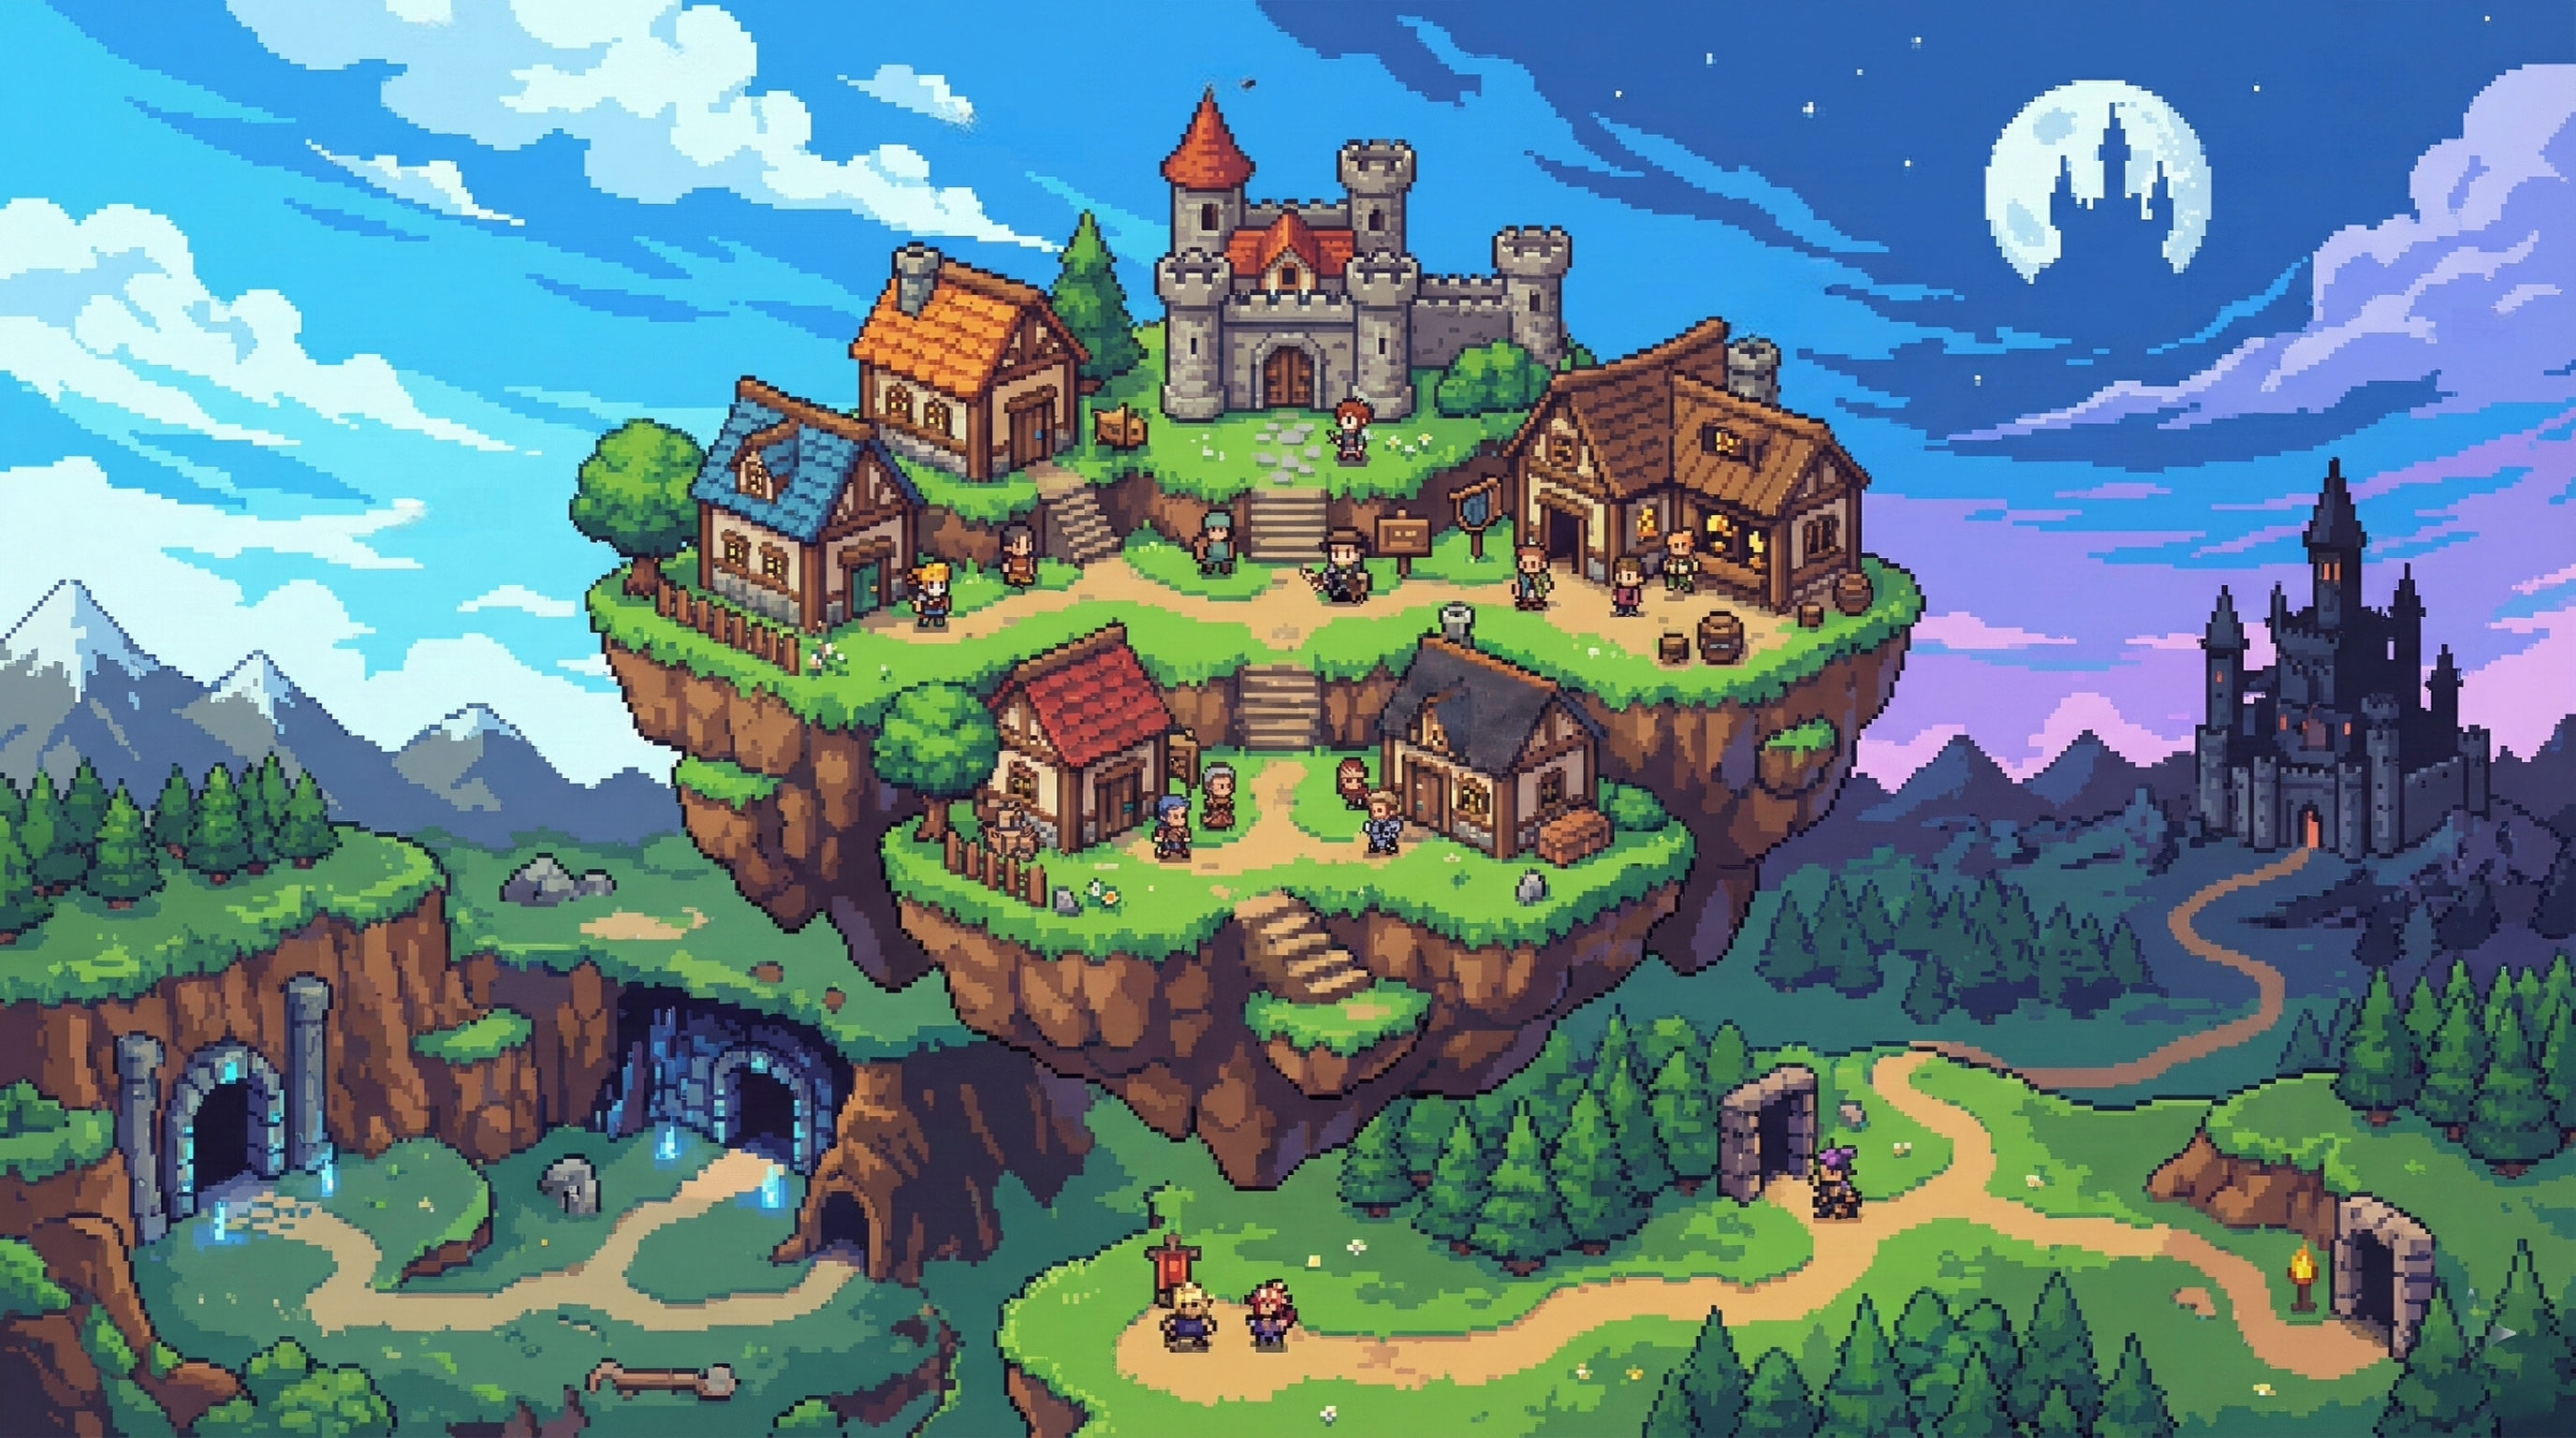
\includegraphics[width=\textwidth]{Images/background.png}
    \caption{Minh hoạ bối cảnh/\allowbreak pixel art mood của game}
    \label{fig:ui-background-mood}
\end{figure}

\subsubsection{Luồng UI xác thực: Login/\allowbreak Register}
\label{subsubsec:design-ui-auth}

\begin{figure}[H]
    \centering
    \includegraphics[width=0.78\textwidth]{Images/login.jpeg}
    \caption{Màn hình đăng nhập (Login)}
    \label{fig:ui-login}
\end{figure}

\begin{figure}[H]
    \centering
    \includegraphics[width=0.78\textwidth]{Images/register.jpeg}
    \caption{Màn hình đăng ký (Register)}
    \label{fig:ui-register}
\end{figure}

Mapping nghiệp vụ và API:
\begin{itemize}
    \item \textbf{Input validation}: username/\allowbreak password không rỗng; hiển thị lỗi theo mã lỗi chuẩn hoá.
    \item \textbf{Endpoint}: \texttt{/auth/\allowbreak login}, \texttt{/auth/\allowbreak register}; (tuỳ chọn) \texttt{/auth/\allowbreak recover}.
    \item \textbf{Trạng thái UI}: loading khi submit; disable nút khi request đang chạy; thông báo lỗi khi sai mật khẩu/\allowbreak tài khoản bị ban.
\end{itemize}

\subsubsection{Luồng UI profile: Select/\allowbreak Create/\allowbreak Delete}
\label{subsubsec:design-ui-profile}

\begin{figure}[H]
    \centering
    \includegraphics[width=0.95\textwidth]{Images/select_profile.png}
    \caption{Màn hình chọn profile (Select Profile)}
    \label{fig:ui-select-profile}
\end{figure}

\begin{figure}[H]
    \centering
    \includegraphics[width=0.95\textwidth]{Images/create_profile.png}
    \caption{Màn hình tạo profile/\allowbreak nhân vật (Create Profile/\allowbreak Character)}
    \label{fig:ui-create-profile}
\end{figure}

Mapping nghiệp vụ và API:
\begin{itemize}
    \item \textbf{Endpoint}: \texttt{/profiles} (list/\allowbreak create/\allowbreak select/\allowbreak delete), \texttt{/characters} (create/\allowbreak select/\allowbreak delete).
    \item \textbf{Ràng buộc}: giới hạn số profile/\allowbreak slot; xác nhận trước khi xoá; kiểm tra trùng tên theo policy.
    \item \textbf{Dữ liệu hiển thị}: level/\allowbreak class/\allowbreak race; thông tin preview ngoại hình lấy từ \texttt{CHARACTER.appearance}.
\end{itemize}

\subsubsection{UI Hub và điều hướng phân hệ}
\label{subsubsec:design-ui-hub}

\begin{figure}[H]
    \centering
    \includegraphics[width=\textwidth]{Images/main_UI.png}
    \caption{UI Hub: điều hướng Inventory/\allowbreak Heroes/\allowbreak Battle/\allowbreak Gacha/\allowbreak Quests}
    \label{fig:ui-main-hub}
\end{figure}

Mapping nghiệp vụ và API:
\begin{itemize}
    \item \textbf{Inventory}: REST tải \texttt{INVENTORY} + \texttt{CHARACTER\_EQUIPMENT} để render chỉ số và item/\allowbreak slot.
    \item \textbf{Heroes}: REST tải \texttt{NPC\_COLLECTION}.
    \item \textbf{Battle}: bắt đầu bằng REST (chuẩn bị data/\allowbreak kiểm tra điều kiện), sau đó chuyển sang WebSocket để realtime.
    \item \textbf{Gacha}: REST tải banner/\allowbreak rates, thực hiện summon, nhận kết quả và cập nhật NPC collection.
\end{itemize}

\subsubsection{UI Inventory/\allowbreak Equipment}
\label{subsubsec:design-ui-inventory}

\begin{figure}[H]
    \centering
    \includegraphics[width=\textwidth]{Images/inventory.jpg}
    \caption{UI Inventory: phân loại item, thao tác Use/\allowbreak Equip và hiển thị currency}
    \label{fig:ui-inventory}
\end{figure}

Mapping nghiệp vụ và API:
\begin{itemize}
    \item \textbf{Inventory tabs}: All/\allowbreak Equip/\allowbreak Use/\allowbreak Mat tương ứng filter theo \texttt{CONFIG\_ITEM.type}.
    \item \textbf{Endpoint}: \texttt{/inventory} (get/\allowbreak use), \texttt{/equipment} (get/\allowbreak equip/\allowbreak unequip), (tuỳ chọn) \texttt{/equipment/\allowbreak enhance}, \texttt{/equipment/\allowbreak repair}.
    \item \textbf{Ràng buộc}: kiểm tra slot trống; kiểm tra \texttt{max\_stack}; thao tác equip/\allowbreak unequip phải nhất quán giữa INVENTORY và CHARACTER\_EQUIPMENT.
\end{itemize}

% ==============================================================
\subsection{Thiết kế vòng lặp real-time cho combat/\allowbreak instance}
\label{subsec:design-realtime}

\subsubsection{Mô hình instance/\allowbreak room}
\label{subsubsec:design-room}

Hệ thống tổ chức người chơi theo \textbf{room} (đơn vị logic của một instance). Mỗi room có:
\begin{itemize}
    \item danh sách người chơi tham gia (socket id, character id);
    \item trạng thái runtime (vị trí, HP/\allowbreak MP, trạng thái skill, entity trong phòng);
    \item cấu hình phiên (mode: tower/\allowbreak dungeon/\allowbreak arena; floor/\allowbreak seed).
\end{itemize}

\subsubsection{Tick loop và phát snapshot}
\label{subsubsec:design-tick}

Thiết kế loop ở mức khái niệm:
\begin{enumerate}
    \item Thu thập input queue từ client.
    \item Xác thực input (cooldown, tài nguyên, vị trí hợp lệ, tốc độ).
    \item Cập nhật trạng thái authoritative theo tick.
    \item Phát snapshot định kỳ và phát event khi có thay đổi quan trọng (hit/\allowbreak loot/\allowbreak death).
\end{enumerate}

Trong giai đoạn 1, cơ chế snapshot có thể thiết kế theo hướng \textbf{đơn giản và rõ ràng}:
\begin{itemize}
    \item snapshot theo tick rate cố định (ví dụ 10--20 tick/\allowbreak s tuỳ mục tiêu kiểm thử);
    \item payload snapshot ưu tiên các giá trị tối thiểu để render (pos, hp/\allowbreak mp, state flags, cast state);
    \item chưa bắt buộc triển khai đầy đủ prediction/\allowbreak reconciliation, nhưng định dạng message chừa chỗ cho mở rộng \cite{gaffer-networking,moriarty-networked}.
\end{itemize}

% ==============================================================
\subsection{Thiết kế phân hệ Administration}
\label{subsec:design-admin}

Phân hệ admin phục vụ quản trị vận hành và kiểm soát rủi ro:
\begin{itemize}
    \item \textbf{Ban/\allowbreak Unban user}: cập nhật \texttt{USER.status}; thu hồi phiên đang hoạt động.
    \item \textbf{System mail}: gửi thông báo/\allowbreak phần thưởng theo user/\allowbreak profile; xử lý qua job để kiểm soát retry.
    \item \textbf{View logs}: truy vấn log theo thời gian/\allowbreak actor/\allowbreak severity; hỗ trợ điều tra sự cố.
    \item \textbf{Configure events/\allowbreak config}: quản trị cấu hình sự kiện và cấu hình gameplay theo phân quyền.
\end{itemize}

Các thao tác admin phải có:
\begin{itemize}
    \item phân quyền theo role;
    \item audit log đầy đủ (ai làm, làm gì, khi nào, trước/\allowbreak sau);
    \item cơ chế chống thao tác lặp gây cấp trùng phần thưởng (idempotent key).
\end{itemize}

% ==============================================================
\subsection{Bảo mật, nhất quán và quan sát hệ thống}
\label{subsec:design-nfr}

\subsubsection{Bảo mật}
\label{subsubsec:design-security}

Các nguyên tắc:
\begin{itemize}
    \item mật khẩu lưu dạng hash; không lưu plaintext;
    \item token có thời hạn; khi ban user cần thu hồi session;
    \item phân quyền rõ giữa player và admin (role-based);
    \item giới hạn tần suất login/\allowbreak gacha và kiểm tra input realtime để chống spam.
\end{itemize}

\subsubsection{Nhất quán dữ liệu và giao dịch nghiệp vụ}
\label{subsubsec:design-consistency}

Các thao tác như reward, gacha, exchange, equip/\allowbreak unequip, nâng cấp công trình/\allowbreak kỹ năng cần đảm bảo:
\begin{itemize}
    \item \textbf{atomic ở mức tài liệu} (MongoDB document update) khi cập nhật trong cùng thực thể;
    \item \textbf{idempotency} cho request dễ bị gửi lại (retry do mạng);
    \item \textbf{log nghiệp vụ} để có thể đối soát và khôi phục khi lỗi.
\end{itemize}

\subsubsection{Quan sát hệ thống (observability)}
\label{subsubsec:design-observability}

Thiết kế log tối thiểu:
\begin{itemize}
    \item request log: endpoint, latency, status code, user id (nếu có);
    \item business log: gacha result, reward delivery, currency delta, equip/\allowbreak skill-up actions, admin actions;
    \item realtime log: join/\allowbreak leave room, disconnect, lỗi xác thực socket.
\end{itemize}

% ==============================================================
\subsection{Tổng kết chương}
\label{subsec:design-summary}

Chương này đã mô tả thiết kế hệ thống ở mức kiến trúc, mô-đun, dữ liệu, giao tiếp và UI/\allowbreak UX tham chiếu cho \textit{Fortress of the Fallen}. Thiết kế nhấn mạnh ranh giới trách nhiệm client--server theo hướng server-authoritative, tổ chức backend theo mô-đun rõ ràng, tách dữ liệu tiến trình khỏi dữ liệu cấu hình, và xây dựng pipeline quản trị cấu hình theo hướng data-driven. Phần thiết kế dữ liệu đã cập nhật ERD (inventory/\allowbreak equipment/\allowbreak skills) và bổ sung data dictionary có caption để các bảng được đánh số và xuất hiện trong danh sách bảng. Các quyết định thiết kế này là nền tảng để mô tả hiện thực hệ thống và kiểm thử trong các chương tiếp theo \cite{nest-docs,mongodb-guide,redis-in-action,gaffer-networking,moriarty-networked}.
